
\documentclass[12pt,a4paper,headsepline,bibliography=totoc,idxtotoc,DIV12,openright,twoside=true,chapterprefix=on]{scrbook} %draft zum Schluss
\renewcommand*{\chapterheadstartvskip}{\vspace*{5cm}} %rausnehmen scrbook
% optional: oneside
%\pagestyle{myheadings}

%\markright{Basics}
\addtokomafont{pageheadfoot}{\linespread{1}\selectfont}
%\usepackage[T1]{fontenc} % Windows
\usepackage{ucs}
\usepackage[rflt]{floatflt}
\usepackage[german]{babel}
\usepackage{siunitx}
\usepackage{color}
%\usepackage[latin1]{inputenc} % Windows
\usepackage[utf8x]{inputenc}
\usepackage{ulem}
\usepackage{amsmath,amssymb}
\usepackage{amsthm}
%\usepackage{mathtools}
%\usepackage[dvips]{graphicx}
\usepackage{graphicx}
%\usepackage[demo]{graphicx}
\usepackage{caption}
\usepackage{subcaption}

\usepackage{bm}

\usepackage{wrapfig}
\usepackage{sidecap}
\usepackage{multirow}
\usepackage{pgf}
\usepackage{tikz}
\usetikzlibrary{arrows,automata}
%\usepackage{pgf}
\usepackage{subfig}
\usepackage[inline]{fixme}
%\usepackage[justification=raggedright,singlelinecheck=false]{caption}
\usepackage{nicefrac}
\usepackage{setspace}
\usepackage{dcolumn}
%\usepackage{ragged2e}
\usepackage{caption}
\captionsetup{format=plain,indention=0cm}
\usepackage[sort,nocompress]{cite}
%\usepackage{achicago}
%\usepackage[authoryear,square]{natbib}
\usepackage{hyperref}
\hypersetup{colorlinks=true, citecolor=black, filecolor=black, linkcolor=black, urlcolor=black}
\onehalfspacing
\usepackage{mathpazo}
\usepackage{todonotes}
\usepackage{setspace}
\usepackage{booktabs}
\usepackage[stable]{footmisc}

\usepackage[autostyle]{csquotes}

\usepackage[
    backend=biber,
    style=authoryear-icomp,
    sortlocale=de_DE,
    natbib=true,
    url=false,
    doi=true,
    eprint=false
]{biblatex}

\addbibresource{~/bibliography/MasterThesis.bib}

\usepackage[]{hyperref}
\hypersetup{
    colorlinks=true,
}

\setlength{\emergencystretch}{1em}

\setlength{\parindent}{0pt} %Unterbindet das Einrücken

\renewcommand{\proofname}{Beweis}

\theoremstyle{definition}
\newtheorem{defi}{Definition}
\newtheorem{bem}[defi]{Bemerkung}
\newtheorem{bsp}[defi]{Beispiel}
\theoremstyle{plain}
\newtheorem{satz}[defi]{Satz}
\newtheorem{theorem}[defi]{Theorem}
\newtheorem{lem}[defi]{Lemma}
\newtheorem{kor}[defi]{Korollar}

\newcommand*\dif{\mathop{}\!\mathrm{d}}
\newcommand*\Dif{\mathop{}\!\mathrm{D}}
\newcommand{\pdn}[2][]{\frac{\partial#1}{\partial#2}}


\newcommand{\IR}{\mathbb{R}}
\newcommand{\IB}{\mathbb{B}}
\newcommand{\IN}{\mathbb{N}}
\newcommand{\IC}{\mathbb{C}}
\newcommand{\re}{\mathrm{Re}} % Realteil
\newcommand{\im}{\mathrm{Im}} % Imaginärteil
\newcommand{\Bi}{\mathrm{im}} % Bild
\newcommand{\spec}{\mathrm{spec}}
\newcommand{\Id}{\mathrm{Id}}
\newcommand{\p}{\mathrm{P}}
\newcommand{\sg}{\mathrm{sgn}}
\newcommand{\Eig}{\mathrm{Eig}}
%\newcommand{\l}{\lambda}
%\newcommand{\t}{\tau}

%\newcommand{\todo}{\fixme[inline]}
\newcommand{\rg}{\text{rank}}
\newcommand{\sgn}{\text{sgn}}
\newcommand{\M}{\text{M}}
\newcommand{\codim}{\text{codim }}
\newcommand\rP{\text{r}}
\newcommand\teMSE{\text{MSE}_{\text{test}}}
\newcommand\trMSE{\text{MSE}_{\text{train}}}
\newcommand\vMSE{\text{MSE}_{\text{val}}}
\newcommand\MCC{\text{MCC}}
\newcommand\Pvalue{\text{p-value}}
%\DeclarePairedDelimiter\set{\lbrace}{\rbrace}

\usepackage[explicit]{titlesec}
\usepackage{xcolor}
\usepackage{lipsum}% just to generate text

\titleformat{\section}[block]
  {\Large}{\thesection.~#1}{1em}{}
  \titleformat{\subsection}[block]
  {\large}{\thesubsection.~#1}{1em}{}
  %\titlespacing*{\subsection}{0pt}{15pt}{10pt}
  \titlespacing*{\section}{0pt}{25pt}{20pt}

%\colorlet{myrulecolor}{black}
\definecolor{myrulecolor}{RGB}{13,105,154}% define the color for the rules

\titleformat{\chapter}[display]
  {\normalfont\scshape\Huge}
  {\hspace*{0pt}\thechapter.~#1}
  {-15pt}
  {\hspace*{-110pt}{\color{myrulecolor}\rule{\dimexpr\textwidth+80pt\relax}{3pt}}\Huge}
\titleformat{name=\chapter,numberless}[display]
  {\normalfont\scshape\Huge}
  {\hspace*{0pt}#1}
  {-15pt}
  {\hspace*{-110pt}{\color{myrulecolor}\rule{\dimexpr\textwidth+80pt\relax}{3pt}}\Huge}
\titlespacing*{\chapter}{0pt}{0pt}{30pt}


\newenvironment{abstract}{\rightskip1in\itshape}{}
%\titleformat{\section}[hang]{\Large\scshape}{\thesection}{1em}{}

%\bibliographystyle{apalike}





\begin{document}

\makeatletter
\renewcommand*\env@cases[1][1.2]{%
  \let\@ifnextchar\new@ifnextchar
  \left\lbrace
  \def\arraystretch{#1}%
  \array{@{}l@{\quad}l@{}}%
}
\makeatother

\begin{titlepage}
       %\vspace*{1cm}
       \begin{center}
       \begin{huge}
       %\textbf{Verzweigung in Netzwerken\\[9mm]}
       \textsc{Titel Thesis auf Deutsch}
       \rule{0.9\textwidth}{0.4pt}\\
       \textsc{Titel Thesis in english\\[1.8cm}
       %\textsc{Auditory information processing in Orthopteran insects \\[2cm]}% processing of auditory mating cues .... temporal mating
       \end{huge}
       \begin{large}
	Masterarbeit\\[2cm]
% 	to obtain the academic degree\\
% 	Doctor rerum naturalium (Dr. rer. nat.)\\[2cm]

	geschrieben am Institut für Geophysik\\
	der Georg-August Universität Göttingen\\[2cm]
	%submitted to the Department of Biology, Chemistry and Pharmacy\\
% 	of Freie Universität Berlin\\[3cm]
       \end{large}
       \begin{large}
       von\\[.5cm]
       Jonas Ruebsam\\
       aus Hildesheim\\
       \vfill
       \begin{center}
       2015
       \end{center}
       \end{large}
     \end{center}
\end{titlepage}

\mbox{}
\thispagestyle{empty}
\newpage
\newpage
\pagenumbering{roman}
\thispagestyle{empty}
\vfill
\noindent \textbf{Die Arbeit wurde im Zeitraum vom XXXX 2014 bis XXXX 2015 in der Arbeitsgruppe "`Fluiddynamik"'
 unter der Betreuung von Prof. Dr. Andreas Tilgner angefertigt. }\\
%
% The research presented in this dissertation was carried out from August 2010\\
% until March 2014 at the Theoretical Neuroscience \& Neuroinformatics
% group, Freie Universität Berlin, under the supervision of Prof.~Dr.~Martin Nawrot.}\\
\vfill
\begin{tabbing}
  \hspace{3cm}\=\kill
   Erstgutachterin: \quad  Prof. Dr. Andreas Tilgner - Universität Göttingen\\
   Zweitgutachter: \quad  Prof. Dr. X Y - Universität Göttingen\\
\end{tabbing}

\newpage
\mbox{}
\thispagestyle{empty}
\newpage
% \mbox{}
% \thispagestyle{empty}
% \newpage
% thispagestyle{empty}

% \vfill
% \noindent Date of defense:
% \vfill
% \vfill
% \vfill

%%%%%%%%%%%%%%%%%%%%%%%%%%%%%%%%%%%%%%%%%%%%%%%%%%%%%%%%%%%%%%%%%%%%%%%%%%%%%%%%%%%%%%%%%%%%%%%%%%%%%%%%%%%%%%%%%%%%%%%%%%%%%%%%%%%%%%%%%%%%%%%%
%%%%%%%%%%%%%%%%%%%%%%%%%%%%%%%%%%%%%%%%%%%%%%%%%%%%%%%%%%%%%%%%%%%%%%%%%%%%%%%%%%%%%%%%%%%%%%%%%%%%%%%%%%%%%%%%%%%%%%%%%%%%%%%%%%%%%%%%%%%%%%%%
% \newpage


% \newpage
% \thispagestyle{empty}
% \vspace{3cm}
% Für meine Eltern, Helga Meckenhäuser und Wolfram Seidel...
% \newpage
% \thispagestyle{empty}
% \mbox{}
% \section*{Acknowledgements}
% First of all, I would like to thank my supervisor Martin Nawrot for the opportunity to work in his interdisciplinary and multicultural research group, for his continuous support, encouragement and openness towards new projects during the past years.
% \newline
% \newline
% I express my gratitude to my experimental collaborators: Matthias Hennig for introducing me to the fascinating world of crickets, for collecting the data for the first project and his clear thoughts for the manuscript; Stefanie Krämer for confiding me to her data from grasshoppers and her patience; Bernhard Ronacher for his ideas and support for finishing the second manuscript. Thanks for providing me with real neuroscientific data!
% \newline
% \newline
% Thanks to all my colleagues. In particular, I want to thank Farzad Farkhooi without whom I would have been stuck in the last year: thanks for the numerous encouraging discussions and helpful remarks on my second project. I also thank Jan Soelter for discussing artificial neural networks over and over again, Thomas Rost for installing packages I could not install, Chris Häusler for his relaxing mood, Michael Schmuker for taking care of Bommel, Evren Pamir for his critical view, Rinaldo Betkiewicz for not loosing control in the polish Milchbar, Joachim Haenicke for his handcreme, and Tara Dezhdar for being a great office mate.
% \newline
% \newline
% I thank Yulia Oganian and Joachim Haenicke how helped to polish this thesis during the final weeks and Florian Rau who never got tired of correcting my writings about crickets and grasshoppers.
% \newline
% \newline
% Many thanks go to my ``ladies'' from Berlin and friends from Hamburg for sharing laughter and tears. Thank you so much for your moral support and love.
% \newline
% \newline
% I dedicate this thesis to my parents Helga Meckenhäuser and Wolfram Seidel to whom I am so grateful for their endless support and encouragement.
%
%
% %irst of all, I would like to thank Martin Nawrot for supervising my PhD project.
%
% \newpage
% \mbox{}
% \thispagestyle{empty}
% \newpage
%
% \newpage
% \thispagestyle{plain}
% \noindent\textbf{This dissertation is based on the following two manuscripts:}
% \vfill
% cricket MS
% \subsubsection*{Critical song features for auditory pattern recognition in crickets}
% \textit{Authors:}\\
% Gundula Meckenhäuser$^{1}$, R.~Matthias Hennig$^{2}$, Martin P.~Nawrot$^{1}$\\
% \textit{Author contributions:}\\ %Research idea by GM, RMH, MPN. Experiments by RMH, Analysis by GM, Manuscript by GM, Revision of the manuscript by MPN, RMH
% GM, RMH, MPN conceived the reseach idea. RMH designed the experiment. \\
% GM analyzed the data. GM, MPN wrote the manuscript. RMH revised the manuscript.\\
% %\\
% %\textit{Acknowledgments:} We thank Jan Clemens, Florian Rau, Jan Sölter, and Thomas Rost for fruitful discussion.\\
% \textit{Manuscript status:}\\ Manuscript has been published in PLoS ONE: doi: 10.1371/journal.pone.0055349 %\citep{Meckenhauser2013}
%
%
%
% grasshopper MS
% \bigskip
% \subsubsection*{Decoding of calling songs and their behavioral relevance from grasshopper auditory neurons}
% \textit{Authors:} \\
% Gundula Meckenhäuser$^{1,*}$, Stefanie Krämer$^{2,*}$, Farzad Farkhooi$^{1}$, Bernhard Ronacher$^{2}$, Martin P.~Nawrot$^{1}$\\
% \textit{Author contributions:} \\
% SK, BR designed the experiments. SK carried out the experiments. GM, FF, MPN developed ideas for data analysis. SK analyzed behavioral data. GM analyzed behavioral and electrophysiological data. GM, SK, BR, MPN wrote the manuscript. FF revised the manuscript.\\
%  %E.P. designed the research, collected and analyzed the data, developed the framework
% %and the model, run the simulations, wrote the paper; J.H. developed the model and revised
%  %the paper; M.N. developed the model and revised the paper;\\
%  %\textit{Acknowledgments:} We thank Michael Schmuker for helpful comments on this work. \\
% \textit{Manuscript status:} \\
% Manuscript has been submitted to Frontiers in Systems Neuroscience on March, 14th, 2014.
%
% \vfill
% \vfill
% \noindent\textbf{Author affiliations:}\\
% $1$ Theoretical Neuroscience \& Neuroinformatics, Institute of Biology, Department of Biology, Chemistry and Pharmacy, Freie Universität Berlin\\
% $2$ Behavioural Physiology Group, Department of Biology, Humboldt-Universität zu Berlin\\
% \bigskip
% $*$ equal contribution
%
% \newpage
% \mbox{}
% \thispagestyle{empty}
%
% \newpage
% \mbox{}
% \thispagestyle{empty}
%
% \thispagestyle{plain}
% \section*{Zusammenfassung}
%
%
% Nanocomposite materials are commonly used in many different applications due to their unique combinations of material properties.
% Here, we try to understand the mechanism of fracture in nanocomposites and the influences of interfaces on fracture in order to learn
% how to separate nanoscale materials efficiently. We study multilayer systems consisting of polycrystalline titanium and amorphous zirconium
% oxide. In order to test the length scale dependent behavior of fracture, we vary the layer thicknesses from 10 nm to 100 nm. The multilayers
% are deformed by using a specially designed in-situ setup inside a TEM with a STM holder.
%
% \vspace{2cm}
% \section*{Summary}
%
% Nanocomposite materials are commonly used in many different applications due to their unique combinations of material properties.
% Here, we try to understand the mechanism of fracture in nanocomposites and the influences of interfaces on fracture in order to learn
% how to separate nanoscale materials efficiently. We study multilayer systems consisting of polycrystalline titanium and amorphous zirconium
% oxide. In order to test the length scale dependent behavior of fracture, we vary the layer thicknesses from 10 nm to 100 nm. The multilayers
% are deformed by using a specially designed in-situ setup inside a TEM with a STM holder.
%
% \vfill
% \vfill
%
%
%

%%%%%%%%%%%%%%%%%%%%%%%%%%%%%%%%%%%%%%%%%%%%%%%%%%%%%%%%%%%%%%%%%%%%%%%%%%%%%%%%%%%%%%%%%%%%%%%%%%%%%%%%%%%%%%%%%%%%%%%%%%%%%%%%%%%%%%%%%%%%%%%%
%%%%%%%%%%%%%%%%%%%%%%%%%%%%%%%%%%%%%%%%%%%%%%%%%%%%%%%%%%%%%%%%%%%%%%%%%%%%%%%%%%%%%%%%%%%%%%%%%%%%%%%%%%%%%%%%%%%%%%%%%%%%%%%%%%%%%%%%%%%%%%%%
% %%%%%%%%%%%%%%%%%%%%%%%%%%%%%%%%%%%%%%%%%%%%%%%%%%%%%%%%%%%%%%%%%%%%%%%%%%%%%%%%%%%%%%%%%%%%%%%%%%%%%%%%%%%%%%%%%%%%%%%%%%%%%%%%%%%%%%%%%%%%%%%%
% \noindent\textbf{Keywords:} \\
% insect acoustic communication, neural information processing, pattern recognition, artificial neural network, na\"{\i}ve Bayes classifier
%
 %classical conditioning, insect brain,
 %honeybee, associative learning, plasticity, neuronal computation, computational modeling
%\input{titlepage}
%\setcounter{tocdepth}{1}
\setcounter{secnumdepth}{3}
%\newpage
\setcounter{page}{1}
\addtocontents{toc}{\protect\setstretch{1.15}}
\tableofcontents

\cleardoublepage

%\newpage
%\thispagestyle{empty}
%\mbox{}
%\thispagestyle{empty}
\setcounter{page}{1}
\pagenumbering{arabic}
\chapter{Theoretische Grundlagen}

\section{Einleitung}

Eine numerische Modellierung setzt zunächst eine exakte theoretische Beschreibung des strömungsmechanischen Problems vorraus.
Daher soll in diesem Abschnitt auf die theoretischen Grundlagen der Strömungsmechanik eines inkompressiblen Fluids eingegangen werden.
Anschließend werden die Grundgleichungen für verschiedene Systeme erweitert die im Laufe dieser Arbeit betrachtet wurden.
Dazu gehört die Strömung in rotierenden Systemen sowie das Rayleigh-Benard-System.

\section{Die Navier-Stokes Gleichung}
I was often using any of the available “lorem ipsum”
I was often using any of the available “lorem ipsum”

\subsection{jawohl}
I was often using any of the available “lorem ipsum”
I was often using any of the available “lorem ipsum”

\chapter{Numerical Methods}

\section{Introduction}

This chapter focuses on the methods that are used for the numerical computations in this thesis.
In order to compute the temporal evolvement of a fluid system from its initial state, it is necessary to discretize
the equations of motion by using different numerical schemes.\\
For this purpose various discretization approaches, for example finite element and finite volume methods, exist.
Here the method of finite differences will be introduced for the spatial discretization and a third order Runge-Kutta method for the temporal discretization in time.
Furthermore we will introduce the method of artificial compressibility, which can be used to avoid the numerical expensive solution of a poisson equation.
The choice of these methods in combination with the usage of cartesian grids is in particular time saving when performing computations on the GPU, as we
will see in chapter \ref{chapter:cuda}.

\section{Finite Differencing Schemes}

We start with a brief introduction of finite difference methods.
The interested reader is referred to \citep{ferziger99} for a more general overview, which this section is based on.
The partial differential equations we want to solve in this thesis are of the generalized form

\begin{align}
    \label{numerik:pde_allg}
    \pdn[\Phi]{t} = \left(\sum_{i=1,2,3}\left( A_i \pdn[]{x_i}  + B_i \pdn[^2]{x_i^2}\right) + C +  \vec{u}\vec{\nabla} \right) \Phi =: \mathcal{L} \Phi
\end{align}
    %\pdn[\Phi]{t} = A \pdn[^2\Phi]{x^2}  + B \pdn[^2\Phi]{x^2}     + C(\vec{r}, \vec{u}, t) +  \vec{u}\left(\pdn[^2\Phi]{x^2} +  \pdn[^2\Phi]{x^2} + \pdn[\Phi]{x}\right) = \mathcal{L}

where $\Phi(\vec{r}, t)\in\mathbb{R}$ and $\mathcal{L}$ is a differential operator, containing spatial derivatives up to second order.
The numerical integration can be divided into two steps: the calculation of $\mathcal{L}$, which we want to discuss in this
section and secondly the integration in time.

The exact calculation of the spatial derivatives in $\mathcal{L}$ is numerically not possible.\\
Due to the limited storage capacity and computation time of computers,
it is necessary to discretize the domain, on which the PDE should be solved and find a adequate approximation of these operators.
Here we will fall back to the  one-dimensional case, the implementation for three dimensions will be discussed in chapter \ref{chapter:cuda}.\\

Let $\Omega = \{x \in \mathbb{R} \;|\; 0 \leq x \leq L\}$ be the domain on which we want to solve equations of the type \ref{numerik:pde_allg}.
For the discretization we divide $\Omega$ into $N$ equidistant points $x_i = \sum_i \Delta x_i$, with the position index ${i\in\{[0, N-1]|i\in\mathbb{N}\}}$
and $\Delta x_i = x_{i+1} - x_i = L/(N-1)$.
\footnote{EVTL?}
We assume that $\Phi$ is a  continuous differentiable function.
Local to a grid point $x_i$ and $\Phi$ can than be expressed with a Taylor series [CITE].

\begin{align}
    \label{num:taylor}
    \Phi(x) = \sum_{n=0}^{\infty} \pdn[^n\Phi(x_i)]{x^n} \frac{(x - x_i)^n}{n!}
\end{align}

By evaluating the Taylor expansion at different points, we obtain expressions for the first derivative. For example
a combined evaluation at the points $x_{i+1}$, $x_{i-1}$ leads to the expression

\begin{align}
    \label{num:cds}
    \left.\left(\pdn[\Phi]{x}\right)\right|_{i} = \frac{\Phi_{i+1} - \Phi_{i-1}}{x_{i+1} - x_{i-1}}
     - \frac{(x_{i+1} - x_i)^2 - (x_i - x_{i-1})^2}{2 (x_{i+1} - x_{i-1})}\left(\pdn[^2\Phi]{x^2}\right)_i + \mathcal{O}(\Delta x^3)
\end{align}

For a constant grid size, that is $\Delta x := \Delta x_i = \text{const.}$, the second order term in equation \ref{num:cds} vanishes.
By neglecting all terms of higher order, we obtain a approximation for $\partial_x \Phi$ of second order.
This is the so-called central-difference (CDS) scheme. A single point evaluation of \ref{num:taylor} at $x_{i+1}$ and $x_{i-1}$, results in the forward- (FDS) and
backward- (BDS) scheme of first order. A comparison of the FD-schemes is given in table \ref{num:df_table}


\bgroup\large
\begin{table}[!tbp]
\centering
\def\arraystretch{2.2}%
\begin{tabular}{c c c c c}\toprule
Scheme-Name & Stencil & Truncation Error & Evaluation at\\[0.5ex]
\midrule
Forward  (FDS) & $\left(\pdn[\Phi]{x}\right)_i =  \frac{f_{i+1} - f{i}}   {\Delta x}$ & $\mathcal{O}(\Delta x)$  &$x_{i+1}$\\
Backward (BDS) & $\left(\pdn[\Phi]{x}\right)_i = \frac{f_{i}    - f_{i-1}}{\Delta x}$  &$ \mathcal{O}(\Delta x)$ & $x_{i-1}$\\\
Central  (CDS) & $\left(\pdn[\Phi]{x}\right)_i = \frac{f_{i+1}  - f_{i-1}}{2\Delta x}$ &$ \mathcal{O}(\Delta x^3)$& $x_{i+1}$ \& $x_{i-1}$\\
\\
\bottomrule
\label{num:df_table}
\end{tabular}
\caption{Different FD-Schemes}
\end{table}
\egroup

\begin{figure}[!btp]
  \centering
    \resizebox{0.9\textwidth}{!}{
   \import{gfx/numerik/}{finite_differenzen.pdf_tex}
  }
  \caption{Approximation of the function $\Phi$ by different finite difference schemes.}
  \label{num:fd_image}
\end{figure}

The numerical error which is made by neglecting the higher order terms, is in general referred to as the truncation error of a FD-scheme.
It should be noted that the number of grid points used for the approximation, does significantly affect the resulting error.\\
Finally figure \ref{num:fd_image} shows a visual comparison for the three different stencils.
This example once again illustrates that when approximating a function, which contains higher order terms i.e. at a local maximum,
the  CDS-scheme gives better results.\\
For the computation of the second derivative, one approach is to evaluate equation \ref{num:taylor} halfway between two points at the positions $x_{i\pm\frac{1}{2}}$

\begin{align}
    \label{numerik:eq_2dfo2}
    \left.\left(\pdn[^2\Phi]{x^2}\right)\right|_{x_i} =
     \frac{\left.\left(\pdn[\Phi]{x}\right)\right|_{i+\frac{1}{2}}-
     \left.\left(\pdn[\Phi]{x}\right)\right|_{i-\frac{1}{2}}}
    {\frac{1}{2}(x_{i+1} - x_{i-1})} + \mathcal{O}(\Delta ^2)  \approx
    \frac{\Phi_{i+1} - 2\Phi_i + \Phi_{i-1}}{\Delta x^2}
\end{align}

For the approximation of the first derivatives, it is necessary to use the FDS-scheme at $x_{i+1/2}$ and the BDS-scheme at $x_{i-1/2}$ to obtain
a second order accuracy.\\
So far we introduced methods up to an accuracy of second order. The fourth order methods which are used in this thesis are given by

\begin{align}
    \left(\pdn[\Phi]{x}\right)_i &\approx \frac{-\Phi_{i+2} + 8\Phi_{i+1} - 8\Phi_{i-1} + \Phi_{i-2}}{12\Delta x} \\
    \left(\pdn[^2\Phi]{x^2}\right)_i &\approx \frac{-\Phi_{i+2} + 16\Phi_{i+1} -30\Phi_i + 16\Phi_{i-1} - \Phi_{i-2}}{12\Delta x^2}
    \label{num:fd_o4_methods}
\end{align}

The derivation of these equations can be performed in analogy to the second order schemes, but by using a five-point
stencil. The interested reader is referred to \citep{Fornberg1988}.

\newpage

\section{Runge-Kutta Method}
\label{numerik:rk_williamson_sec}

With the finite difference approximation $\mathcal{L^*}$ of the differential operator $\mathcal{L}$,
we are able to solve equation \ref{numerik:pde_allg} by separation of variables.

\begin{align}
    \Phi(t) = \Phi(0) + \int_{t_0}^{t} \mathcal{L^*} (t, \Phi(t)) \dif t
\end{align}

For a numerical computation, the integration interval $[t_0, t]$  is splitted into sub-intervals $[t^n, t^{n+1}]$ of length $\Delta t$ and integrated piecewiese.
In order to approximate the integration on a sub-intervall, we know want to introduce the use of Runge-Kutta methods based on \citep{Sarbach2012}
The idea behind this method is to iteratively evaluate $\mathcal{L^*}$ at $s$ different times $\tau_i=c_i \Delta t$ with $c_i \in \{\mathbb{R} | c_i<1  \}$,
that is
\begin{align}
 k_i = \mathcal{L^*} \left(\tau_i, \Phi(t_n) + \Delta t \left(a_{21} k_{s-1} + \dots + a_{s, s-1} k_{s-1} \right)\right)
\end{align}

By using a coefficient weighted average of the $k_i$, we obtain

\begin{align}
    \Phi(t^{n+1}) = \Phi(t) + \Delta t \left( \sum_{i=1}^s b_i k_i \right)
\end{align}

The accuracy of an s-stage runge-kutta method depends of the right choice of coefficients.
In this thesis we use a third-order accurate scheme.
The coefficients are given by the butcher tableau \citep{QUELLE}
\footnote{oder quelle}

\begin{align}
    \label{num:butcher}
    \def\arraystretch{1.5}%
    \begin{array}{c|c}
        \mathbf{c} & A\\
        \hline     & \mathbf{b^T} \\
    \end{array}
    \qquad &= \qquad
    \def\arraystretch{1.5}%
    \begin{array}{c|ccc}
            0 \\
                    \frac{1}{3} & \frac{1}{3} \\
            \frac{3}{4} & \frac{-3}{16} & \frac{15}{16} \\
            \hline & \frac{1}{6} & \frac{3}{10} & \frac{8}{15}
    \end{array}
\end{align}

For the implementation of this method, we have to concern, that we have to deal with a large number of variables.
In a three dimensional fluid domain the number of grid points scales with a power of three, with an increase in the resolution.
Therefore we want to introduce a low-storage scheme of method \ref{num:butcher},  first introduced by \citep{Williamson1980}.
By keeping the information from previous computation steps, the scheme can than be translated into an iterative algorithm,
where the required amount of storage can be reduced to two registers $\Phi$ and $Q$.

\begin{align}
    \begin{split}
    Q_1 = \Delta t \mathcal{L}^*\left(\Phi^n\right)\qquad &\Rightarrow \qquad \Phi^{1} = \Phi^n + \frac{1}{3}Q_1 \\
    \Rightarrow Q_2 = \Delta t \mathcal{L}^*\left(\Phi^1\right) - \frac{5}{9} Q_1 \qquad &\Rightarrow \qquad \Phi^{2} = \Phi^1 + \frac{15}{16}Q_2 \\
   \Rightarrow  Q_3 = \Delta t \mathcal{L}^*\left(\Phi^2\right) - \frac{153}{128} Q_2 \qquad &\Rightarrow \qquad \Phi^{n+1} = \Phi^2 + \frac{8}{15}Q_3 \\
    \end{split}
\end{align}


\section{Numerical Stability}

It is important to consider the stability of a numerical method. In general it is said that a method is numerical stable if the error
introduced by approximations and roundoff errors does not grow over time \citep{ferziger99}.\\

\subsection{Runge-Kutta Scheme}

Suppose we have stationary solution for equation \ref{numerik:pde_allg}.
The system should remain unaffected by a further integration, even with the introduction of small numerical errors.
In order to obtain a stability condition it is sufficient enough to perform a linear stability analysis.
The most common approach is to study the one-dimensional linearized and diagonalized test problem (\citep{BLABLA})

\begin{align}
\label{num:rk_stab}
\frac{\dif y}{\dif t} = \lambda \Phi
\end{align}

with the eigenvalue $\lambda \in \mathbb{C}$ of a linearized operator.
It can be shown that the discretization of equation \ref{num:rk_stab}, using a Runge-Kutta scheme of $s$-order,
results in  the mapping (\citep{BLABLA})

\begin{align}
    y_{i+1}  = \left(\sum_{p=1}^s \frac{(\Delta t \lambda)^p}{p!}  + 1 \right) y_i = f(\Delta t\lambda)y_i
\end{align}

\begin{figure}[!tp]
  \begin{minipage}[c]{0.6\textwidth}
      \includegraphics{gfx/numerik/rk_stability.pdf}
  \end{minipage}\hfill
  \begin{minipage}[c]{0.3\textwidth}
  \caption{Stability regions for $\Omega_s$ for different Runge-Kutta methods}
  \label{fig:num_rkstab}
  \end{minipage}
\end{figure}

The discretized system contains a stable fixed point when the condition $|f|\leq 1$ is satisfied.
Figure \ref{fig:num_rkstab} shows the different stability regions for Runge-Kutta schemes up to fourth order.
The calculation can be found in (APPENDIX)
For an $s$ order scheme the region of absolute stability is independent of the used implementation \citep{canuto2007}.
\footnote{For an $s$-th order RK-scheme different coeffiicent $a_ij$, $b_j$ and $c_i$ can be used.}
It can be noted that the stability region $\Omega_s$ increases with the uses of higher order schemes.
The substantial detail is that for method of third and fourth order, the imaginary axis lies within $\Omega_s$.
Thus these methods should be preferred for  CFD-simulations, since they tend to stabilize numerical oscillations \citep{DIPLOM}.

\subsection{Finite difference schemes}

The numerical stability of the finite difference schemes can be estimated by a Von-Neumann error analysis.
In this section the stability criterion will be exeplarily computed for a one-dimensional diffusion equation of the form
\begin{align}
    \label{num:vne_diffusion_theo}
    \pdn[v]{t} = \alpha \Delta v
\end{align}

where $\alpha$ is the diffusion coefficient. Eq.  \ref{num:vne_diffusion_theo} is discretized by
the second order central-difference scheme, given by Eq. \ref{numerik:eq_2dfo2}.
All methods and steps in this example are adopted from \citep{janderson}.
In order to test if a method is stable, it is valid to assume that the numerical error can be expressed in form of a fourier-mode.

\begin{align}
    \epsilon(x, t) = \sum_{m=1}^{N/2} \epsilon_m(x, t) \qquad &\text{and} \qquad  \epsilon_m(x, t) = e^{at}e^{i k_m x}
\end{align}

where $a$ the growth rate of the error, the wavenumber is given by $k_m=\nicefrac{2\pi m}{L}$ and $L$ is the size of the simulation domain.
The index $m$ is restricted by the domain size and the distance $\Delta x$ between two grid points, i.e. the smallest wave number
is resulting from the wavelength $\lambda=L$ and the largest from $\lambda=2\Delta x$.
Due to the linearity of the laplace operator it is sufficient to consider the stability of a single fourier mode $\epsilon_m$.
With the use of Eq.  \ref{numerik:eq_2dfo2}, the discretized version of the diffusion equations reads.
\begin{align}
    \label{num:neumann_diffusion_eq}
    \frac{\Phi^{n+1} - \Phi^n}{\Delta t} = \frac{\alpha}{\Delta x^2}\left(\Phi_{i+1}^n - 2\Phi_{i}^n + \Phi_{i-1}^n\right)
\end{align}

where $\alpha$ is the diffusion coefficient. The timestep in this example is discretized by a simple euler timestep.
Inserting $\epsilon_m$ in Eq. \ref{num:neumann_diffusion_eq} for $\Phi$ and using some trigonometric identities  gives

\begin{align}
    e^{a \Delta t} = 1 -  \frac{4\alpha \Delta t}{\Delta x^2} \sin^2\left(\frac{k_m \Delta x}{2}\right)
\end{align}

Furthermore it holds that

\begin{align}
    \left|\frac{\epsilon_i^{n+1}}{\epsilon_i^n}\right| =
    \left|\frac{e^{a(t + \Delta t)}e^{ik_mx}}{ e^{at}e^{ik_m x}}\right| = \left|e^{a\Delta t}\right|
\end{align}

The stability of the finite differenc scheme is given when the numerical error does not grow over time. This is fullfilled when the inequality

\begin{align}
    \label{num:stab_ineq}
    \left|\frac{\epsilon_i^{n+1}}{\epsilon_i^n}\right| =
    \underbrace{\left|1 -  \frac{4\alpha \Delta t}{\Delta x^2} \sin^2\left(\frac{k_m \Delta x}{2}\right)\right|}_{=:G} \leq 1
\end{align}

holds, where $G$ is denoted as the amplification factor. From the inequality from Eq. \ref{num:stab_ineq}
the stability is given by

\begin{align}
   \frac{\alpha \Delta t}{\Delta x^2} \leq \frac{1}{2}
\end{align}

From this equation it can be seen that with an increase in the resolution, the timestep has to been scaled by the square of the resolution, in order to
maintain stability. The same approach introduced for the diffusion equation can be repeated for a first-order wave equation (see \citep{janderson})
and for an advection-diffusion equation (see \citep{ferziger99}).
%Given by
%\begin{align}
%    \pdn[\Phi]{t} + c \pdn[\Phi]{x} = 0 \qquad &; \qquad  \pdn[\Phi]{t} + v \pdn[\Phi]{x}  - \frac{A}{B}\pdn[^\phi]{x^2}
%\end{align}
%where $c$ is velocitiy ect.
%By inserting the error

As a result two additional stability criterions are given.
The first one is (see \citep{janderson})
\begin{align}
    \label{num:stab_soundspeed}
   \frac{c \Delta t}{\Delta x} \leq 1
\end{align}
where $c$ denotes the maximal velocity of the system, i.e. this could be the sound speed for a compressible system.
The second criterion is given by (see \citep{ferziger99}

\begin{align}
    \Pe  < 2
\end{align}

where $ Pe := \nicefrac{u \Delta x}{\alpha}$ is defined as the Peclet number \citep{ferziger99}.
The Peclet number can be interpreted as the ratio between the advection and diffusion of a fluid system.

\paragraph{Third Order Upwinding Scheme}\mbox{}\\

For large Peclet numbers it is a common problem that numerical oscillations emerge in the numerical solution.
Additional to the central differences, the upwinding scheme, which tends to reduce
numerical oscillations, is used in this thesis. Consider the one-dimensional advection equation

\begin{align}
    \pdn[\Phi]{t} + v\pdn[\Phi]{x} = 0
\end{align}

The discretization for the advection term at the position $x=i$ is given by (see \citep{FINDQUOTE})

\begin{align}
    v\pdn[\Phi]{x} &\approx  v_i \cdot \left(\frac{2\Phi_{i+1} + 3\Phi_i     - 6\Phi_{i-1} + \Phi_{i-2}}{6\Delta x}\right)\\
\end{align}
for v(x) > 0 and
\begin{align}
    v\pdn[\Phi]{x} &\approx  v_i \cdot \left( \frac{-\Phi_{i+2} + 6\Phi_{i+1} - 3\Phi_{i-1} - 2\Phi_{i-1}}{6\Delta x}\right)
\end{align}
for v(x) < 0.

\newpage

\section{Numerical Viscosity}

In this thesis the finite difference schemes Eq.  \ref{num:fd_o4_methods} and Eq.  \ref{numerik:eq_2dfo2}
are used for the approximation of the viscous stress in the Navier-Stokes Equation.
However due to the approximation, the numerical viscosicty $D_N$ of the approximation may differ from the physical viscosity $D_P$.
An estimation for the ratio $D_N/D_P$ can be given by the following estimation. \footnote{Private communication with A.Tilgner}
Consider the  equation

\begin{align}
    \label{num:nvis_eqdiff}
    \pdn[v]{t} = D_P\pdn[^2v]{x^2}
\end{align}

A solution is given by $v = V(t)e^{ikx}$. Inserting this solution in Eq. \ref{num:nvis_eqdiff} one obtains
\begin{align}
    V(t) = V_0 \exp^{-D_Pk^2t}
\end{align}

By inserting this expression into the second order approximation Eq. () it
follows that

\begin{align}
                      D_P \Delta v  &\approx \frac{D_P}{\Delta x^2} \left(v_{x+\Delta x} - 2 v_x + v_{x - \Delta x}\right) \\
    \Leftrightarrow   -D_P k^2        &\approx \frac{D_P}{\Delta x^2} \left(\exp^{ik\Delta x} - 2 + \exp^{-ik\Delta x}\right) =   \frac{D_P}{\Delta x^2} \left(2\cos(k\Delta x) - 2\right)\\
    \Rightarrow   D_P      &\approx - \frac{D_P}{k^2 \Delta x^2} \left(2\cos(k\Delta x) - 2\right)
\end{align}

From Eq. it can be seen that the numerical viscosity is given by
\begin{align}
 \label{NUMERIC:NUMVIS}
    D_N = \frac{D}{k^2 \Delta x^2} \left(2\cos(k\Delta x) - 2\right)
\end{align}
The same approach for the fourth order scheme gives
\begin{align}
 \label{NUMERIC:NUMVIS2}
    D_N = \frac{D}{k^2 \Delta x^2} \left(32\cos(k\Delta ) - 2\cos(k\Delta x) - 30\right)
\end{align}
\clearpage



\section{Method of Artificial Compressibility}

For now the fact was ignored that the Navier-Stokes Eq. \ref{theorie:eqns} cannot directly be solved for the pressure.
An equation for $p$ can be obtained by taking the divergence of Eq. \ref{theorie:eqns} and apply the continuity equation.
The resulting equation is \citep{QUOTE}

\begin{align}
    \Delta p =  -\nabla \left( \sum \vec{F}_{\text{ext.}} - (\vec{u} \vec{\nabla}) \vec{u}\right)
\end{align}

In order to determine the pressure it would be necessary to solve a poisson equation.
The numerical solution  however, can be very time consuming is  furthermore difficult to implement on a GPU \citep{TILGNER}.
Instead here the method of artificial compressibility, developed by \citep{Chorin1997}, will be introduced.
The concept of this method is to introduce the artificial equations of state


   \noindent\begin{minipage}{0.4\textwidth}
        \begin{align}
            \label{num:arti_cont}
            \pdn[\rho]{t} +  \nabla \vec{v} = 0
        \end{align}
    \end{minipage}%
    \begin{minipage}{0.2\textwidth}\centering
        \begin{align}
            \label{num:arti_pressure}
              p =\rho/\delta
        \end{align}
    \end{minipage}%
    \begin{minipage}{0.2\textwidth}\centering
        \begin{align}
                c=\frac{1}{\delta^{1/2}}
        \end{align}
    \end{minipage}\vskip1em




where $\rho$ is the artifical density, $\delta$ the artificial compressibility and $c$ the artificial speed of sound.
Eq.  \ref{num:arti_cont}  is a motified version of the continuity equation and Eq. \ref{num:arti_pressure} introduces
an artificial equation for the pressure. A substitution of Eq. \ref{num:arti_pressure} into Eq. \ref{theorie:eqns} gives

\begin{align}
    \label{numerik:nsac}
    \pdn[u]{t} + \left(\vec{u} \vec{\nabla}\right) \vec{u} &= -c^2\nabla\rho + \Rey \Delta \vec{u}+\sum \vec{F}_{\text{ext.}}
\end{align}


The system now has an artificial compressibility. The motivation behind this approach is to set the artifical speed of sound
to a high value such that the mach number given by

\begin{align}
    M = \frac{v}{c} =  \frac{1}{c}\max\left(\sum_i |\vec{u_i}]^2\right)^{1/2}
\end{align}
is small, a good estimation is $Ma<0.1$ \citep{HM}.
In this case the fluid can be considered as incompressible.
One major drawback of this method is a stiff numerical problem. Due to the stability criterion (Eq. \ref{num:stab_soundspeed})
a small timestep is needed for $v=c^2$.





\chapter{GPU Implementierung}

\section{Einleitung}

Nachdem das theoretische und numerische Fundament gelegt wurde, soll nun auf die GPU-Implementierung eingegangen werden.
Dieser Abschnitt bezieht sich auf den grundlegenden Algorithmus, welcher im Rahmen der Master-Arbeit basierend auf einer bestehenden
CUDA-Implementierung von [] übernommen, erweitert und optimiert wurde.
Die zusätzlich eingeführten  Immersed Boundary Methoden werden ausführlich in Abschnitt () behandelt.

\section{GPU Architektur}
- karten varianten c1060 und tesla k20m , datasheet im anhang

-In Abbildung () ist exemplarisch das Speicherlayout der cuda karte dargstellt .
-Hierbei sei angemerkt das dies in keiner weise dem hardware layou entspricht aber als model
-für verständnis der algoritmhus am besten
-z.b. ist der local memory auf der karte im global memory speicherbereich

- lese paper / präsi zur optimierung
- geschwindigkeiten
- shared vs global etc

\begin{figure}[!bp]
  \centering
  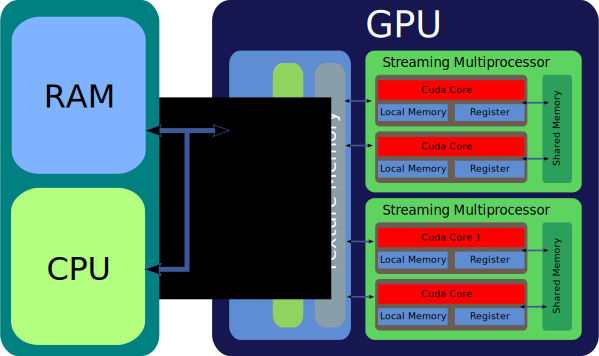
\includegraphics[width=0.8\textwidth]{gfx/cuda/gpu.png}\label{fig:gpu_arch}
  \caption{Speicherlayout einer Nvidia-GPU}
\end{figure}

-bild
-speicher bereiche
-grid layout function call
-threadidx etc

\section{Algorithmus}
-oder so ?
-erläuterung  implementierung
-speicherverwaltung

\section{Optimierung}
- coalesceded
- bank conflicts?
- teilvolumen nicht rechnen

\section{Validierung}
- beispiel rayleigh benard system
- masa
- vgl o2 vs o4 masa cube
- bifurcation


\newpage



\chapter{Immersed Boundary Methods for No-Slip Walls}
\section{Overview of Immersed Boundary Methods}

\begin{figure}[!bp]
  \centering
  \subfloat[cartesian grid]{\includegraphics[width=0.4\textwidth]{gfx/immersed_boundary_methods/general_partition_triangle.jpg}\label{fig:grid_f1}}
  \hfil
  \subfloat[unstructured body-fitted grid]{\includegraphics[width=0.4\textwidth]{gfx/immersed_boundary_methods/general_partition_triangle.jpg}\label{fig:grid_f2}}
  \caption{Different types of numerical grids}
\end{figure}

For many fluid problems it is mandatory to solve the equations of motion with respect to complex-shaped geometries \.
The algorithm introduced in section () is not yet suitable for such a scenario.
For instance the simulation inside a spheric geometry is impossible, since the boundaries
do not coincide with the implemented cartesian grid. Nevertheless there exist different approaches to overcome this problem,
which shall be introduced here. \\
The common approach to extend the algorithm would be to use a body-fitted mesh (see figure \ref{fig:grid_f1}),
different advantages and disadvantages arise with this kind of implementation (see \citep{Mittal2005}).
One benefit is a much simpler deployment of the desired boundary condition, due to the overlap of the grid with domain border.
Furthermore a higher accuracy can be achieved \citep{Gornak2013}.
However, using an unstructered grid generates plenty of computational overhead, during and before the execution of a simulation.
The generation of the grid is very complicated in contrast to using a cartesian grid, this can be even more complicated when
considering moving boundaries.
Also solving the finite differenc schemes on a curvilinear coordinate system, leads to more calculations on a single grid point.
The last important aspect is the implementation on the gpu.
Like discussed in section () it is more efficient to use homogenous storage and calculation pattern on a CUDA-device,
the use of unstructured data makes this very difficult.
Altough some attempts exists to solve these difficulties (see i.e. PAP), it is still uncertain if the obtained performance loss would be acceptable.\\
A set of alternative methods, to resolve the problems described above, are so called Immersed Boundary Methods.
The term was first mentioned in (PESKIN 1972), for the simulation of blood flow through a heartvale, but has since then been used for a variety of
methods (MITTAL).  All of them have the idea in common to perform the simulations on a cartesian grid which does not conform to the domain boundary.
To satisfy the desired boundary conditions additional terms are introduced into the equations of motion.
In general one can distinguish between contiuous forcing methods and direct forcing methods.
Continious forcing methods try to mimic the boundary using a localized force which acts on the boundary,
since the surface is tracked by lagrangian points this methods can be well suited for moving boundaries (MITTAL).
One common problem is that continous forcing can arise to stability problem and numerical oscillations in numericial stiff problem (SOURCE).
The direct forcing approach tries to satisfies the boundary condition, by imposing it directly to points near the fluid surface for example
trough an interpolaltion procedure.
Some of the major drawbacks using the IBM is the loss in  spatial accuracy at the boundary, therefore it can be necessary to use a higher grid resolution
compared to a body-fitted mesh.  Futhermore the non-conforming (?) boundaries are more difficult implement.
The benefits of these methods is the use of a cartesian grid, which is much more suited for a gpu-based implementation (see section X).
As a result the overall performance will probably be in the same order as the original algorithm.
In the thesis the Implementation of different Immersed Boundary Methods is seperated into three chapters depending on the boundary condition and application.
This chapter beginns with Implementation of NoSlip-Walls which are the easisest to implement.
The term Immersed Boundary Method is vaguely defined in literature, in this thesis we refer to it with all methods introduced in the following three chapters.

\newpage

\section{IBM-Methods}
\section{Volume Penalization}

%Die Volume-Penalization Methode ermöglicht es, durch einen Kraftterm der auf die einzelnen Fluidzellen wirkt, mit wenig Aufwand Noslip-Ränder zu implementieren.
%Das Verfahren wurde in mehreren Publikationen z.B. [bla] erfolgreich verwendet, eine mathematisch exaktere Abhandlung lässt sich z.B. in [bla2] finden.
%
%\begin{wrapfigure}{r}{0.5\textwidth}
%  \begin{center}
%  \includegraphics[width=0.5\textwidth]{gfx/immersed_boundary_methods/mask.png}\label{fig:mask_vp}
%  \includegraphics[width=0.5\textwidth]{gfx/immersed_boundary_methods/mask.png}\label{fig:mask_vp}
%  \end{center}
%  \caption{Maskierungsfunktion $H(x,y,z=const.) = x^2 + y^2 < c$ für einen Zylinder. }
%\end{wrapfigure}
%
%Das Volumen wird zunächst in einen Fluidbereich und einen festen Wandbereich, wie in Abb.1 dargestellt, unterteilt. Für die Differenzierung der Bereiche während der Simulation wird  eine Maskierungsfunktion
%\begin{align}
%H(x, y, z) = \begin{cases}
%                    0, & \text{für } \vec{x}(x,y,z) \in Fluid, \\
%                    1, & \text{sonst}.
%             \end{cases}
%\end{align}
%verwendet. Als zusätzlicher Kraftterm wird nun eine exponentielle Dämpfung eingeführt die nur auf den Wandbereich des Volumens wirkt.
%\begin{align}
%\vec{f} = \frac{H(x, y, z)}{\nu}(\vec{v} - \vec{v_0})
%\end{align}
%Bei $\vec{v_0}$ handelt es sich um die gewünschte Randbedingung, der Kraftterm ist also proportional zur Auslenkung $\vec{v}$ eines Punktes vom gewünschten Ruhezustand.
%Die Antwort des Kraftterms wird durch die Dämpfungrate $\nu$ reguliert. Je kleiner $\nu$ desto stärker ist die Dämpfungsrate, allerdings kann der Term
%nicht beliebig klein gesetzt werden da die Stabilität für $\nu < dt$ nicht mehr gewährleistet ist [source].
%Da für die Lösung der der Geschwindingskeitsfelder mit der Methode der künstliche Kompressibilität  bereits ein sehr kleiner Zeitschritt verwendet wird (s.Abb. X)
%kann im Vergleich zu anderen Verfahren wie z.B. (pseudo-spektrale) eine relativ starke Dämpfungsrate verwendet werden.
%
%\subsubsection{Validierung mit MASA}
%-validierung mit masa für alle verfahren oben.. cube /evtl zylinder?
%-vegl. und argumentation ränder ehh auf null.
%-ein beispiel mit vol.pen.
%
%\subsubsection{Validierung : planare Poiseuille Strömung}
%Es stellt sich die Frage in welcher Größenordnung die Dämpfungskonstante $\nu$ der Volume Penalization methode liegen muss, um einen möglichst kleinen
%Fehler zu gewährleisten. Ein einfacher Testfall der sich hierfür betrachen lässt ist eine einfache planare poiseuille strömung, diese ist schematisch in Abb. (x). dargestellt.
%\paragraph*{Theoretische Beschreibung}\mbox{}\\
%Wir betrachten eine laminare Strömung in x-Richtung die durch einen Druckgefälle $f=-\frac{\partial p}{\partial x}$ angetrieben wird.
%Für die x- und y-Richtung werden periodische Randbedingungen angenommen. In z-Richtung wird das Volumen durch zwei Ebenen bei $h_1$ und $h_2$ begrenzt,
%es gilt $ \vec{v}(z=h_1) = \vec{v}(z=h_2) = 0$.
%Im stationären Fall lässt sich  die Bewegungsgleichung dann  auf eine Dimension reduzieren, es gilt:
%
%\begin{align}
%\frac{\partial v_x}{\partial t} &= - \frac{\partial p}{\partial x} + D \frac{\partial^2 v_x}{\partial z^2} = 0 \\
%\Rightarrow v_x &= \frac{1}{2D}\frac{\partial p}{\partial x}z^2 + zc_1 + c_2\\
%\end{align}
%
%Mit $\vec{v}(h_1) = \vec{v}(h_2) = 0$ und $A:=\frac{1}{2D}\frac{\partial p}{\partial x}$ ergibt sich:
%\begin{align}
%c_1 &= A\frac{h_1^2 -h_2^2}{h_2 - h_1} = -A(h_1+h_2)\\
%c_2 &= A(h_1(h_1 + h_2) - h_1^2) = Ah_1h_2\\
%\Rightarrow v_x &= A(z^2 - z(h_1 + h_2) + h_1h_2)
%\end{align}
%Da die Strömung in der Kanalmitte am stärksten ist gilt zudem:
%\begin{align}
%z_{max} &= \frac{h_1+h_2}{2}\Rightarrow v_{max} = A\left(h_1h_2 - \frac{(h_1 + h_2)^2}{4}\right)
%\end{align}
%Für die Strömung lässt sich die Reynoldszahl dann gemäß $Re \propto \frac{v_{max}}{D}$  bestimmen.
%\begin{figure}[!hbtp]
%  \centering
%  \includegraphics[width=0.9\textwidth]{gfx/immersed_boundary_methods/vp_flow.png}\label{fig:vp_flow}
%  \caption{Geschwindigkeistprofile im Kanal bei Variation der Dämpfungskonstante $\nu$ und Reynoldszahl $Re=500$.}
%\end{figure}
%
%\paragraph*{Setup}\mbox{}\\
%Um die Abhängigkeit des Fehlers von der Dämpfungskonstante zu betrachten wurde ein Kanal mit $l_x=1$, $l_y=1$ und $l_z=2$ sowie $h_1=0.25$, $h_2=0.75$.
%betrachtet. Die Maskierungsfunction ergibt sich damit gemäß $H(z) = (z>h1) \wedge (z<h2)$.
%Für die Reynoldszahl wurden Werte im Intervall $Re \in [100, 500]$ verwendet, die Dämpfungskonstante wurde zwischen $\nu \in [1e-5, 0.1]$ variert, während der Zeitschritt mit $dt =1e-5$ konstant gehalten wurde. Die genauen Angaben für alle Parameter sind in (Anhang Tab.X) zu finden.
%
%\paragraph*{Ergebnisse}\mbox{}\\
%Zunächst ist in Abb. \ref{fig:vp_flow} das Geschwindigkeitsprofil der Strömung für $Re=500$ exemplarisch dargstellt. Es lässt sich bereits qualitativ sehr gut erkennen, dass für eine
%starke Dämfung die Kanalströmung an den Grenzen $h_1$ und $h_2$ verschwindet und gut mit der dem theoretischen Profil übereinstimmt.
%Bei einem Verringern der Dämpfungrate entwickelt sich im Rand ein Geschwindigkeitsprofil.
%Um sicherzustellen dass sich das Profil vollständig entwickelt wurde die Simulation bis zu dem Zeitpunkt fortgegeführt
% in welchem die kinetische Energie des Systems einen stationären Wert erreicht. Anschließend wurde der absolute und relative Fehler mit Formel (X) berechnet,
%dabei wurde das theoretische Profil gemäß () verwendet. Die Ergebnisse sind in Abbildung \ref{fig:vp_error} dargestellt.
%
%\begin{figure}[!bp]
%  \centering
%  \includegraphics[width=1.0\textwidth]{gfx/immersed_boundary_methods/vp_error.png}\label{fig:vp_error}
%  \caption{Absoluter und relativer Fehler in Abhängigkeit von Dämpfungskonsante $\nu$ und Reynoldszahl $Re$.}
%\end{figure}
%
%Bei beiden Fehler lässt sich ein Abfall bis $\nu=1e-4$ erkennen, anschließend kommt es zu einem minimalen Anstieg.
%Betrachtet man den absoluten Fehler, so fällt auf das im Bereich $\nu>5\cdot10^{-3}$, mit steigender Reynoldszahl, der Fehler zunimmt.
%Dies entspricht zunächst der Erwartung, da das Geschwindigkeitsprofil mit steigender Reynoldszahl stärker an der Wand zerrt.
%Allerdings kommt es im Bereich $\nu \in [1e-3 - 1e-2]$ zu einem umgekehrten Verhalten, der Fehler nimmt mit der Reynoldszahl ab,
%Du Ursache hierfür liess sich nicht eindeutig klären.
%Für den relativen Fehler lässt sich ein Abfall mit steigender Reynoldszahl beobachten. Da $\vec{f} \propto (\vec{v}-\vec{v_0})  \propto Re$ wird der Reibunsterm
%proportional zur Reynoldszahl skaliert. Der Fehler durch den Rand ändert sich, im Vergleich zum Geschwindigskeitsprofil kaum, wodurch der Abfall zustande kommt.
%Der relative Fehler fällt bei $\nu=1e-4=10\Delta t$ auf unter 1\%, wodurch dieser Wert als geeignet angesehen werden kann für zukünftige Simulationen mit der Volume-Penalization Methode.
%
%-todo: fluktuation im rand
%
%
%\subsection{Direct Forcing Methode}
%Während die Volume Penalization Methode die Geschwindigkeit ausserhalb des Volumens nicht vollständig auf Null setzt,
% kann dies durch eine implizite Berechnung des Dämpfungsterm erreichtwerden. Es stellt sich heraus das dieser Ansatz equivalent
%  zu der Direct Forcing Methode ist, die erstmals von [] verwendet und in [] beschrieben wird.
%Betrachten wir zunächst den diskretisierten Zeitschritt
%\begin{align}
%    \frac{\vec{u}^{n+1} -\vec{u}^n}{\Delta t} = \mathscr{L} + \vec{f}\\
%\end{align}
%wobei $\mathscr{L}$ den diskretiesierten Operatoren der PDE entspricht.
%Für einen Punkt auf dem Rand des Volumens soll nun die Randbedingung $\vec{u}^{n+1} = \vec{u}_0$ eingehalten werden.
%Mit Formel () folgt
%\begin{align}
%    \frac{\vec{u}_0 -\vec{u}^n}{\Delta t} = \mathscr{L} + \vec{f} \Rightarrow \vec{f} = \frac{\vec{u}_0 -\vec{u}^n}{\Delta t\cdot \mathscr{L}}\\
%\end{align}
%Mit der Annahme dass der Rand mit dem numerischen Gitter übereinstimmt ist es nicht nötig den Kraftterm zur berechnen, stattdessen lässt sich der
%Schritt vereinfachen in dem der Randwert nach  jedem Zeitschritt direkt auf die gewünschte Randbedingung gesetzt wird. Durch die
%implizite Behandlung kommt es zu keiner weiter Stabilitätsbedingung.
%Analog zur Volume-Penalization Methode wurde eine Serie von Simulationen für eine planare Poiseuille-Strömung durchgeführt.
%Das Setup enstpricht dem gleichen wie in Abschnitt (X), lediglich das Verfahren wurde entsprechend angepasst und es wurden finite Differenzen Verfahren zweiter und
%vierter Ordnung getestet.
%In Abbildung () ist der relative Fehler, im Vergleich zur Volume Penalization  Methode mit $\nu=1e-4$ dargestellt.
%Für das Verfahren vierter Ordnung liegt der Fehler im Bereich von 1\% und ist im Mittel doppelt so groß wie für die Volume-Penalization Methode.
%Der Fehler für das Verfahren zweiter Ordnung verschwindet hingegen nahezu.
%Das Verhalten lässt sich durch die Verwendung unterschliedlicher Schablonen, wie in Abb() dargestellt,  der finiten differenzen Verfahren erklären.
%Während das Verfahren zweiter Ordnung nur den Randpunkt sieht, liegt bei der vierten Ordnung ein Punkt innerhalb des Randes.
%Da auch dieser Wert auf Null gesetzt wird, kommt es zu einem fehler in der Berechnung von $\nabla u$.
%
%\begin{figure}[!tpb]
%  \centering
%  \includegraphics[width=0.6\textwidth]{gfx/immersed_boundary_methods/dfo2o4.png}\label{fig:df_o2o4}
%  \caption{bla}
%\end{figure}
%
%-Zeitserie
%
%-einleitung gekrümmte geometrien
%
%\subsection{Direct Forcing mit Volume Fraction}
%-paper quote formeln
%-implementierung beispiel
%
%\section{Direct Forcing mit Interpolation}
%-paper quote formeln
%-implementierung beispiel
%
%\section{Methoden-Vergleich und numerische Validierung}
%In diesem Abschnitt sollen die verschiedenen Methoden über numerische Testfälle validiert und miteinnander
%verglichen werden.
%
%
%\subsubsection{Poiseuille Strömung im Zylinder}
%
%\subsubsection{Zusammenfassung}
%
%
%\subsection{No-Flux-Boundaries}
%
%\subsubsection{'Variable Konduktivität'}











\newpage
\thispagestyle{empty}
\mbox{}

% \newpage
% \thispagestyle{empty}
% \mbox{}l
% %\cleardoublepage


\printbibliography

% \chapter*{Danksagung}

\begin{otherlanguage}{ngerman}
  \thispagestyle{empty}





  \null\vfill
  \noindent
\end{otherlanguage}

\end{document}
